\chapter{Random Variables}
\label{fundamentals}

In this Chapter some basic concepts, that will be used throughout the remaining part of this notes, are reviewed.

\section{Random Variable}
\label{random-variables}

In probability and statistics a random variable is described as a variable whose values depend on outcomes of a random phenomenon. 
It can be formalized as a certain function that is defined over the set of all possible outcomes, referred to as sample space \(\Omega\). 

For example, in the event of a coin toss, only two outcomes 
are possible: heads or tails. 
If instead the random variable is designated to represent the sum of the resulting numbers after 
three dice are rolled, it could be 3 ($1 + 1+ 1$), 18 ($6 + 6 + 6$), or somewhere between 3 and 18, 
since the highest number of a die is 6 and the lowest is 1.

Since in all cases that are taken into account here, \(X\) is real-valued, formally a random variable can be understood as a measurable function defined on a probability space 
that maps from the sample space to the real numbers.
If \(X\) denotes a random variable

\begin{equation}
X:\Omega \rightarrow E
\end{equation}
where \(E=\mathbb {R}\), or in words, \(E\) represents the set of real numbers. 

A random variable's possible values might represent the possible outcomes of a yet-to-be-performed experiment. They may also conceptually represent either the results of an "objectively" random process (such as rolling a die). As a function, a random variable is required to be measurable, which allows for probabilities to be assigned to sets of its potential values. 

A random variable is different from an algebraic variable. The variable in an algebraic equation is an unknown value that can be calculated. The equation $10 + x = 13$ shows that we can calculate the specific value for $x$ which is 3. On the other hand, a random variable has a set of values, and any of those values could be the resulting outcome.

In the corporate world, random variables can be assigned to properties such as the average price of an asset over a given time period, the return on investment after a specified number of years, the estimated turnover rate at a company within the following six months, etc. Risk analysts assign random variables to risk models when they want to estimate the probability of an adverse event occurring. 

When the range of possible values for \(X\) is un-countably infinite then \(X\) is called a \emph{continuous random variable} and its distribution can be described by a \emph{probability density function} (PDF). Contrary if the range is countable, the random variable is called a \emph{discrete random variable} and its distribution can be interpreted as a discrete probability distribution.

A PDF is a function whose values at any given sample, within the set of all possible values taken by the random variable, can be interpreted as providing a relative likelihood that the value of the random variable would equal that sample. Left plot in Fig.~\ref{fig:pdf_pmf} shows an example of gaussian probability density function.

In a more precise sense, the PDF is used to specify the probability of the random variable falling 
within a particular range of values. The probability density function is non-negative everywhere, and its integral over the entire space is equal to 1.
In the context of discrete random variables the probability density function is usually referred 
to as \emph{probability mass function} (PMF). Right plot in Fig.~\ref{fig:pdf_pmf} shows an example of discrete probability density function.

\begin{figure}[htb]
	\centering
	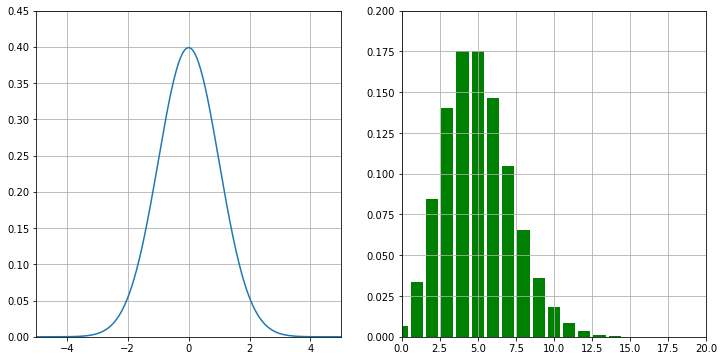
\includegraphics[width=1.\textwidth]{figures/pdf_pmf.png}
	\caption{On the left an example of continuous probability density function (Normal), on the right a discrete probability mass function (Poissonian).}
	\label{fig:pdf_pmf}
\end{figure}

\subsection{Cumulative Distribution and Quantile Functions}\label{sec:quantile-function}

The \emph{cumulative distribution function} (CDF) \(F\) of a random variable \(X\), 
evaluated at \(x\), is the probability that \(X\) will take a value less than or equal to \(x\)

\begin{equation}
	F_X(x) = P(X \le x)\qquad\mathrm{or~equivalently}~\int_{-\infty}^{x}{f(X)dX}
\end{equation}
so it gives the area under the probability density function \(f\) from
minus infinity to \(x\).
The probability that \(X\) lies in the interval \((a,b]\) is therefore

\begin{equation}
	P(a\lt X \le b)=F_{X}(b)-F_{X}(a)\qquad\mathrm{or}~\int_a^b{f(X)dX}
\end{equation}
Notice that by the previous definition any random variable can be conveniently described by its 
cumulative distribution too.

The quantile function $Q$, associated with a probability distribution of a random variable, specifies the value $x$ of the random variable such that the probability $p$ of the variable being less than or equal to that value equals the given probability. It is also called the percent-point function (PPF) or inverse cumulative distribution.

In terms of the cumulative distribution function \(F\), the quantile function \(Q\) returns the value \(x_p\) such that 

\begin{equation}
F_{X}(x_p)=P(X\le x_p)=p
\end{equation}
So the quantile function does the opposite of the cumulative distribution function: given a probability \(p\) (or a value of the CDF) it returns the \(x\) at which the CDF reaches this probability, so we can write $Q=F^{-1}$.

In Fig.~\ref{fig:percentile} an example related to the Gaussian distribution is shown. On the left side the Gaussian PDF is drawn, the red area representing the 30\% of the total area (which is 1 by definition). On the right the corresponding CDF is represented, in the plot it is highlighted the point at which the CDF reaches 30\%. The corresponding quantile value is also indicated and 
is $-0.5244$.

\begin{figure}[htb]
	\centering
	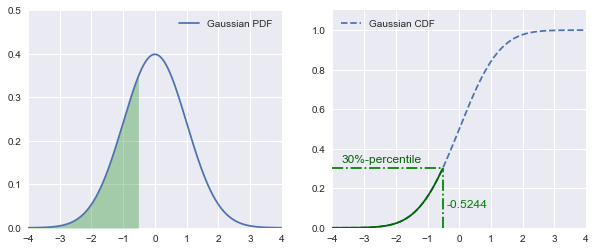
\includegraphics[width=1.\textwidth]{figures/percentile.png}
	\caption{On the left a standard normal distribution, the filled region represent the 30\% of the total area
		under the curve. On the right the corresponding CDF with the 30\% point and the relative quantile highlighted.}
	\label{fig:percentile}
\end{figure}

The computation of CDF and quantiles is quite simple in \(\tt{python}\). The implementation of many distributions is available in \(\tt{scipy.stats}\) module and for each of them the methods \(\tt{cdf(x)}\) and \(\tt{ppf(x)}\) can be used to evaluate CDF and quantile respectively.

\begin{ipython}
from scipy.stats import norm

quantile = norm.ppf(0.3)
cdf = norm.cdf(quantile)
print ("30%-quantile of standard normal is {}".format(quantile))
print ("CDF value at {}: {}".format(quantile, cdf))
\end{ipython}
\begin{ioutput}
30%-quantile of standard normal is -0.5244005127080409
CDF value at -0.5244005127080409: 0.29999999999999993
\end{ioutput}

If instead of a distribution you have a dataset the quantile can be determined using the function \(\tt{numpy.percentile}\) (this will be useful when estimating VaR). Notice that in this case we are talking about \emph{percentile} which is the \emph{quantile} times 100 (e.g. 50-percentile is equivalent to 0.5-quantile).

\begin{ipython}
import numpy
dist = [1, 2, 3, 4, 5, 6, 7, 8, 9]

# first argument the data-set
# second argument a list of percentiles
perc = numpy.percentile(dist, [1, 50])
print (perc)
\end{ipython}
\begin{ioutput}
[1.08 5.  ]
\end{ioutput}

\subsection{Expected Value}\label{sec:expected-value}

In probability theory, the expected value of a random variable \(X\) is a generalization of the weighted average, and is intuitively the arithmetic mean of a large number of independent realizations of \(X\).

\subsubsection{Discrete Case}
Let \(X\) be a random variable with a finite number of finite outcomes \((x_{1},x_{2},\ldots ,x_{k})\) occurring with probabilities \((p_{1},p_{2},\ldots ,p_{k})\) respectively. The expectation of \(X\) is then defined as

\begin{equation}
	\mathbb{E}[X]=\sum _{i=1}^{k}x_{i}\,p_{i}=x_{1}p_{1}+x_{2}p_{2}+\cdots +x_{k}p_{k}
\end{equation}

Since \(p_{1}+p_{2}+\cdots +p_{k}=1\), the expected value is the weighted sum of the \(x_{i}\) values, with weights given by the probabilities \(p_{i}\).

By definition, the expected value of a constant random variable \(X=c\) is \(c\). The expected value of a random variable \(X\) with equiprobable outcomes \((c_{1},\ldots ,c_{n})\) is defined as the arithmetic mean of the terms \(c_i\). 

As an example let \(X\) represent the outcome of a roll of a fair six-sided die. More specifically, \(X\) will be the number of "pips" showing on the top face of the die after the toss. The possible values for \(X\) are 1, 2, 3, 4, 5, and 6, all of which are equally likely with probability \(1/6\).

The expectation of \(X\) is

\begin{equation*}
	\mathbb{E}[X]=1\cdot {\frac {1}{6}}+2\cdot {\frac {1}{6}}+3\cdot {\frac {1}{6}}+4\cdot {\frac {1}{6}}+5\cdot {\frac {1}{6}}+6\cdot {\frac {1}{6}}=3.5
\end{equation*}
If one rolls the die \(n\) times and computes the average (arithmetic mean) of the results, then as \(n\) grows, it will almost surely converge to the expected value.

\subsubsection{Continuous Case}
If \(X\) is a random variable with a probability density function of \(f(x)\), then the expected value is defined as

\begin{equation}
\mathbb{E}[X]=\int_{\Omega}xf(x)dx
\end{equation}
For multidimensional random variables, the expected value is defined per component, that is,

\begin{equation}
\mathbb{E}[(X_{1},\ldots ,X_{n})]=(\mathbb{E} [X_{1}],\ldots ,\mathbb{E}[X_{n}])
\end{equation}

\subsection{Some Properties of Expected Value}\label{some-properties}

\begin{itemize}
\tightlist
\item
Let \(\mathbb{1}_{A}\) denote the indicator function of an event \(A\), then

\begin{equation}
	\mathbb{E}[\mathbb{1}_{A}] = 1\cdot P(A)+0\cdot P(\Omega \setminus A)= P(A)
\end{equation}

\item
the expected value operator \(\mathbb{E}\) is linear in the sense that, for any random variables \(X\) and \(Y\), and a constant \(a\)
\begin{equation}
\begin{cases}
\mathbb{E}[X+Y] = \mathbb{E}[X] + \mathbb{E}[Y] \\
\mathbb{E}[aX] = a\mathbb{E}[X]
\end{cases}
\end{equation}

This means that the expected value of the sum of any finite number of random variables is the sum of the expected values of the individual random variables, and the expected value scales linearly with a multiplicative constant;

\item
the expected value of a measurable function of \(X\), \(g(X)\), given that \(X\) has a probability density function \(f(x)\), is given by 

\begin{equation}
	\mathbb{E}[g(X)] = \int_{\Omega}g(x)f(x) dx
\end{equation}

This formula also holds in multidimensional case, when \(g\) is a function of several random variables, and \(f\) is their joint density;

\item
\(n\) random variables \(X_1 ,\ldots , X_n\) are independent if the following property holds for all positive functions \(f_1 ,\ldots , f_n\)

\begin{equation}
	\mathbb{E}[f_1 (X_1 )\cdots f_n (X_n )] = \mathbb{E}[f_1 ( X_1 )] \cdots \mathbb{E}[f_n (X_n )]
\end{equation}
\end{itemize}


%
%We have seen so far how to generate a sequence of random numbers from U
%{[}0, 1{]}. However, most of the simulations include the sampling of
%random variables, or even random vectors in a mul- tidimensional case,
%from specified, not uniform distributions. Sampling of nonuniform random
%variates is done indirectly, i.e.~one transforms samples from the
%uniform to a desired nonuniform distribution. Accordingly, each
%realization of a nonuniform random variable is directly obtained from a
%single uniform variate or from a sequence of uniforms {[}46, p.54{]}.
%There are numerous algorithms that allow you to generate random numbers
%from a certain desired distribution. However, two main criteria in order
%to choose between them are accuracy and speed.


%
%\hypertarget{correlated-normal-variables-and-vectors}{%
%\subsubsection{Correlated normal variables and
%	vectors}\label{correlated-normal-variables-and-vectors}}
%
%A \(d\)-variate normal distribution \(\phi(\mu, \Sigma)\) is generally
%specified by its mean vector \(\mu\) and variance- covariance matrix
%\(\Sigma\). Random vectors from a multivariate normal distribution can
%be generated directly by generating a \(d\)-vector of iid standard
%normal deviates \(z' = (z_1 , z_2 ,\dots , z_d)\).
%
%Next we know from the linear transformation property that if the vector
%\(z∼\phi_d (0,I)\) and \(x = \mu + Az\), then \(x ∼\phi_d (\mu, AA')\).
%Therefore, we can generate a sequence of univariate normal random
%variables \(z_i\) and put them into a vector \(z\). Thus the challenge
%is merely made up of finding the matrix \(A\) for which the property
%\(AA' = \Sigma\) holds. The representation of \(\Sigma\) as \(AA'\) with
%\(A\) as a lower triangular matrix is denoted as a Cholesky
%factorization of the variance-covariance matrix \(\Sigma\). If
%\(\Sigma\) is symmetric positive definite there is a Cholesky
%factorization and the sampling of multivariate normals is easily done by
%basically sampling from a univariate \(\phi(0,1)\).
%
%In some applications in finance random variables or vectors are required
%to depend on each other in a prescribed way, i.e.~they must not be
%totally uncorrelated. Correlated random variables are calculated
%according to the following algorithm:
%
%\begin{enumerate}
%\def\labelenumi{\arabic{enumi}.}
%\tightlist
%\item
%calculate the Cholesky factorization \(AA′ = \Sigma\),
%\item
%calculate \(z ∼ \phi(0,I)\) by component, for \(i = 1,2,\ldots ,d\),
%\item
%\(x=\mu + Az\), then \(x∼\phi (\mu, \Sigma )\).
%\end{enumerate}
%
%Suppose we have a two-dimensional case, \(d = 2\). Next we are looking
%for a vector \(x' = (x_1 , x_2 ) ∼ \phi (0, \Sigma )\). The correlation
%between \(x_1\) and \(x_2\) is denoted by \(\rho\) and thus the Cholesky
%factorization provides \(\Sigma = AA'\)
%
%\[\begin{bmatrix}
%\sigma_1^2 & \rho\sigma_1 \sigma_2\\
%\rho\sigma_1 \sigma_2 & \sigma_2^2 
%\end{bmatrix} = 
%\begin{bmatrix}
%\sigma_1 & 0\\
%\rho\sigma_2 & \sigma_2\sqrt{1-\rho^2} 
%\end{bmatrix}
%\begin{bmatrix}
%\sigma_1 & \rho\sigma_2 \\
%0 & \sigma_2\sqrt{1-\rho^2} 
%\end{bmatrix}\]
%
%If \(z_1\) and \(z_2\) are independent and from \(\phi(0, 1)\), then
%
%\[\begin{bmatrix}
%x_1\\
%x_2 
%\end{bmatrix} = A
%\begin{bmatrix}
%z_1\\
%z_2 
%\end{bmatrix} = 
%\begin{bmatrix}
%\sigma_1 z_1\\
%\sigma_2 (\rho z_1 + \sqrt{1-\rho^2}z_2) 
%\end{bmatrix}
%\]
%
%are distributed according to \(\phi(0, \Sigma)\).
%
%\begin{codebox}
%\prompt{In}{incolor}{ }{\boxspacing}
%\begin{Verbatim}[commandchars=\\\{\}]
%	
%\end{Verbatim}
%\end{codebox}

\begin{thebibliography}{9}
\bibitem{bib:random_variable}\href{http://www.stat.yale.edu/Courses/1997-98/101/ranvar.htm}{\emph{Random Variables}}, Yale University [Online]
\bibitem{bib:pdf} \href{https://mathinsight.org/probability_density_function_idea}{\emph{The idea of a probability density function}} [Online]
\bibitem{bib:cdf}\href{https://www.probabilitycourse.com/chapter3/3_2_1_cdf.php}{\emph{Cumulative Distribution Function }}, Probability Course [Online]
\bibitem{bib:quantile}\href{https://en.wikipedia.org/wiki/Quantile}{\emph{Quantile}}, Wikipedia [Online]
\bibitem{bib:expected_value}\href{https://www.investopedia.com/terms/e/expected-value.asp}{\emph{Expected Value}}, Investopedia [Online]
\end{thebibliography}